%!TEX root = main.tex

\section{MicroSpark} % (fold)
\label{sec:microspark}

\subsection{Components} % (fold)
\label{sub:components}

\begin{description}
    \item[Driver]
    Driver will visit the lineage of the RDD and split the lineage into different stages. Each stage will be convert to a partition operation object and add in to the stage list. During the execution phrase driver will send the stage object to the workers.
    \item[Worker]
    Worker will management the real data partition, do the transformation and cache the intermedia data. When the worker receive the stage object it will do the transformation to the relevant RDD partition and generate new RDD partitions.
    \item[MacroSparkShell]
    An interactive shell which can submit and run the code directly on the cluster.
    \item[Client]
    Client is the user defined application.
\end{description}

% subsection components (end)

\subsection{Cluster Setup} % (fold)
\label{sub:cluster_setup}
The driver will ssh to different machines and launch different worker processes on it. We can also add new workers through the MacroSparkShell during the execution time. Each time the new workers was added the driver will reset the worker list.
% subsection cluster_setup (end)

\subsection{Failover} % (fold)
\label{sub:failover}
The design of the failover if pretty simple. When a worker failure happened. Drive will reset the cluster and recalculate the RDD using the RDD lineage.
% subsection failover (end)

\subsection{Stage Split} % (fold)
\label{sub:stage_split}
We will split the lineage based on the repartition as showed in Figure~\ref{fig:stage_split}. After the stage split each stage will be a narrow dependency stage except the repartition stage. So we can pipeline the execution for each stage.
\begin{figure}[ht]
    \centering
    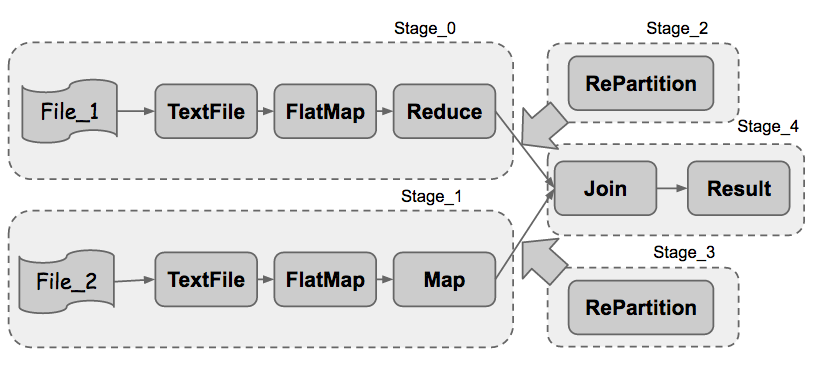
\includegraphics[width=0.45\textwidth]{stage_split.png}
    \caption{Stage Split}\label{fig:stage_split}
\end{figure}
% subsection stage_split (end)

\subsection{Execution} % (fold)
\label{sub:execution}
The real execution process is to transform from one RDD to another and then execute the next transformation. This is fine when we can put all the data into the memory, but when we have a data set that too large to fit into the memory we may meet some problems. We pipeline the execution in each stage so we can put part of our data in memory and do transformation iterations as much as possible.

\begin{figure}[ht]
    \centering
    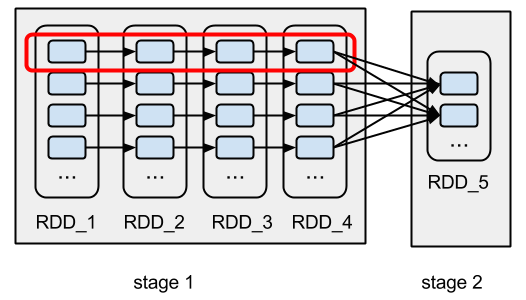
\includegraphics[width=0.45\textwidth]{execution_flow.png}
    \caption{Execution Flow}\label{fig:execution_flow}
\end{figure}

As we can see in Figure~\ref{fig:execution_flow}, we will do all the transformations in the red block for the data in the memory at once, so we don’t need to reload the data when it need to do the transformation from RDD\_2 to RDD\_3 or from RDD\_3 to RDD\_4.
% subsection execution (end)

% section microspark (end)
